\documentclass[a4paper,12pt]{article}
\usepackage{graphicx} 
\usepackage{amsmath} 
\usepackage{amssymb} 
\usepackage{geometry} 
\usepackage{fancyhdr} % for headers and footers
\usepackage{caption} % for customizing captions
\usepackage{subcaption}
\usepackage{setspace} 
\usepackage[bottom]{footmisc}
\usepackage{adjustbox}
\usepackage{placeins}
\usepackage[nopatch=item]{microtype}
\usepackage{enumitem} % for customizing lists
\usepackage[backend=biber]{biblatex} % for bibliography
\usepackage[colorlinks,linkcolor=blue,citecolor=blue,urlcolor=blue]{hyperref}
\addbibresource{Sci. Data_01.bib} % specify your bibliography file

\setlength{\parindent}{1.27cm} % Indent first line of each paragraph by 1.27 cm (0.5 inches)

\geometry{margin=1in}
\setlength{\parindent}{0pt}
\setlength{\parskip}{6pt}
\doublespacing

 
\pagestyle{fancy}
\fancyhf{}
\fancyhead[L]{\leftmark}
\fancyfoot[C]{\thepage}

 
\newcommand{\customtitlepage}{
    

    \begin{titlepage}
        \includegraphics[width=0.9\textwidth]{logo.png}\\
        \centering
        \vspace*{1cm}
        
        \Huge\textbf{A Basic Study of Dimensionality}\\
        \vspace{0.5cm}
        \LARGE\textit{A Quantitative Approach}\\
        \vspace{1.5cm}
        
        \textbf{Scientific Data Acquisition and Processing} \\
        \textbf{Instructors:} Riccardo Barberi, Mario Ferraro\\
        \vspace{0.5cm}
        
        \textbf{Authors:}\\
        \large Michele Arcuri, Luca Coscarelli, Nelson Manuel Mora Fernández\\
        \vfill
        
        \large \textbf{Date of Submission:}\\
        \today\\
        \vspace{1.5cm}
        
        \small
        Department of Physics \\
        University of Calabria\\
        \vspace{0.5cm}
    \end{titlepage}
}

\begin{document}

% Title page
\customtitlepage

% Abstract
\begin{abstract}
This experiment investigates the fractal nature of crumpled aluminum spheres. Initially, we measured the mass and linear 
dimensions of aluminum square sheets, confirming their two-dimensional nature through a power law relationship. Subsequently, 
we rolled these sheets into spheres and measured their diameters and masses to determine their fractal dimensions. 
Despite initial discrepancies, further analysis and exclusion of high-uncertainty data points yielded a fractal dimension between 2 and 3, 
aligning with theoretical expectations. This study demonstrates the fractal characteristics of crumpled aluminum foil and highlights
the importance of precise measurements and data analysis in experimental physics.
\end{abstract}


% Keywords
\section*{Keywords}
fractal, felf-similarity, fractal dimension, Aluminum foil, spheres, curve, fitting, model, regression, power law, linearization, least squares method.
\newpage

% Table of Contents
\tableofcontents
\newpage

% Introduction
\section{Introduction}
\par The following experiment aims to demonstrate the fractal nature 
of a very simple physical object: a small tin foil ball. 
 
\par Fractal objects are characterized by the property of self-similarity; 
in simpler words, they look the same when observed at different scales.
One of the most famous fractal objects is the Mandelbrot set, but other examples can be found 
in nature, such as in the structure of a Romanesco Cauliflower, or, 
from a physical point of view, polymers can be regarded as fractals as well \cite{rubinstein-2003}.

\begin{figure}[h]
    \centering
    \fbox{%
        \begin{minipage}{.8\textwidth} % Adjust the width of the box
            \centering
            % Cauliflower images
            \begin{subfigure}[b]{0.50\textwidth}
                \centering
                \includegraphics[width=0.99\textwidth]{Cauliflower1.jpg}
                \includegraphics[width=0.99\textwidth]{Cauliflower.jpg}
                \caption{Cauliflower from far (top) and up close (bottom).}
                \label{fig:Cauliflower}
            \end{subfigure} 
            \hfill 
            % Mandelbrot images
            \begin{subfigure}[b]{0.485\textwidth}
                \centering
                \includegraphics[width=0.99\textwidth]{Mandelbrot_far.jpg}
                \includegraphics[width=0.99\textwidth]{Mandelbrot_close.jpg}
                \caption{Mandelbrot set from far (top) and up close (bottom).}
                \label{fig:Mandelbrot}
            \end{subfigure}
            
        \end{minipage}%
    }
\end{figure}

\par Another way to describe fractals is by looking at the level of complexity. 
In the images Fig. (\ref{fig:Cauliflower}) and Fig. (\ref{fig:Mandelbrot}) above,
we can observe the complexity level of some of these objects as seen from far away 
and up close.

\par From a mathematical point of view, we define a fractal from its changes 
in terms of mass and volume. For example, we start from an object that we know: 
a square sheet of paper. In this case we will have the mass distributed following the area of 
the sheet, furthermore the mass grows as the square of the typical length of the 
sheet (the side of the square which we call $r$). The formula will be the 
following 
\[ M = C r^2, \]
where $C$ is the surface density of the material of the sheet. We can say that the 
dimension on the sheet of paper is equal to the exponent $2$.

We can repeat the same reasoning with a metal cube, obtaining ultimately the formula
\[ M = D r^3, \]
where $D$ is the volume density of the metal used. It is of course a three-dimensional object.

\par Now, let's apply this idea in our experiment. Since the physical data we 
collect in the laboratory are the mass and the linear dimension of the system 
(the tin foil ball), the unknown parameters will be the general density $k$ and 
the dimensionality exponent $\alpha$, which is the fractal dimension of the system.
\begin{equation} 
    M_{\text{experimental}} = k r_{\text{experimental}}^{\alpha}
    \label{eq:gen_fractal}
\end{equation}   

We anticipate that, in the following experiment, we show how a rolled up ball of 
tin foil can be considered a fractal object, and our main goal will be to determine its fractal dimension.

% Materials and Methods (Tools and Procedure)
\section{Materials and Methods}
\subsection{Equipment and Tools}
\begin{itemize}
    \item Precision balance
    \item Caliber
    \item Micrometer
    \item Drawing rule and square
    \item Scissors
    \item Aluminum foil
\end{itemize}

\subsection{Experimental Procedure}
\label{subsec:exp_procedure}
We begin by checking that we have everything at our disposal. In order to do so, we set up the laboratory as shown in Fig. (\ref{fig:lab_instr}).
Then we start off from the aluminum foil and we cut, using the scissors, a few square sheets of tin foil. 
We had to be careful in cutting squares as perfect as possible in order to reduce the error in 
the measurementes; to do so, we make use of both the ruler and the square. We cut squares of linear 
dimensions of $3$ mm, $5$ mm, $8$ mm, $11$ mm, $14$ mm, $17$ mm, $20$ mm, $23$ mm, $26$ mm and $29$ mm.

\begin{figure}[h!]
    \centering
    \includegraphics[width = 0.55\textwidth]{Lab_instruments.jpg}
    \caption{Our laboratory setup}
    \label{fig:lab_instr}
\end{figure} 

Next, for each square, we measure the mass three times using the precision balance. We also make measurements of the different 
lengths of the square as represented in Fig (\ref{fig:sq_measure}). Finally, we collect all data in an excel spreadsheet which we will show in the next section.

\begin{figure}[h!]
    \centering
    \includegraphics[width = 0.35\textwidth]{square_measure.png}
    \caption{All the direction in which we measured the length of the side of the aluminum foil squares} 
    \label{fig:sq_measure}
\end{figure}

Now, we roll up every tin foil square into a sphere trying to have each ball at the same density as shown in Fig. (\ref{fig:tf_balls}). 
Since we do this operation by hand, we can only have an idea of its density. 
This is the step in the experiment which brings in the maximum amount of error. 

\begin{figure}[h!]
    \centering
    \begin{minipage}{0.45\textwidth}
        \centering
        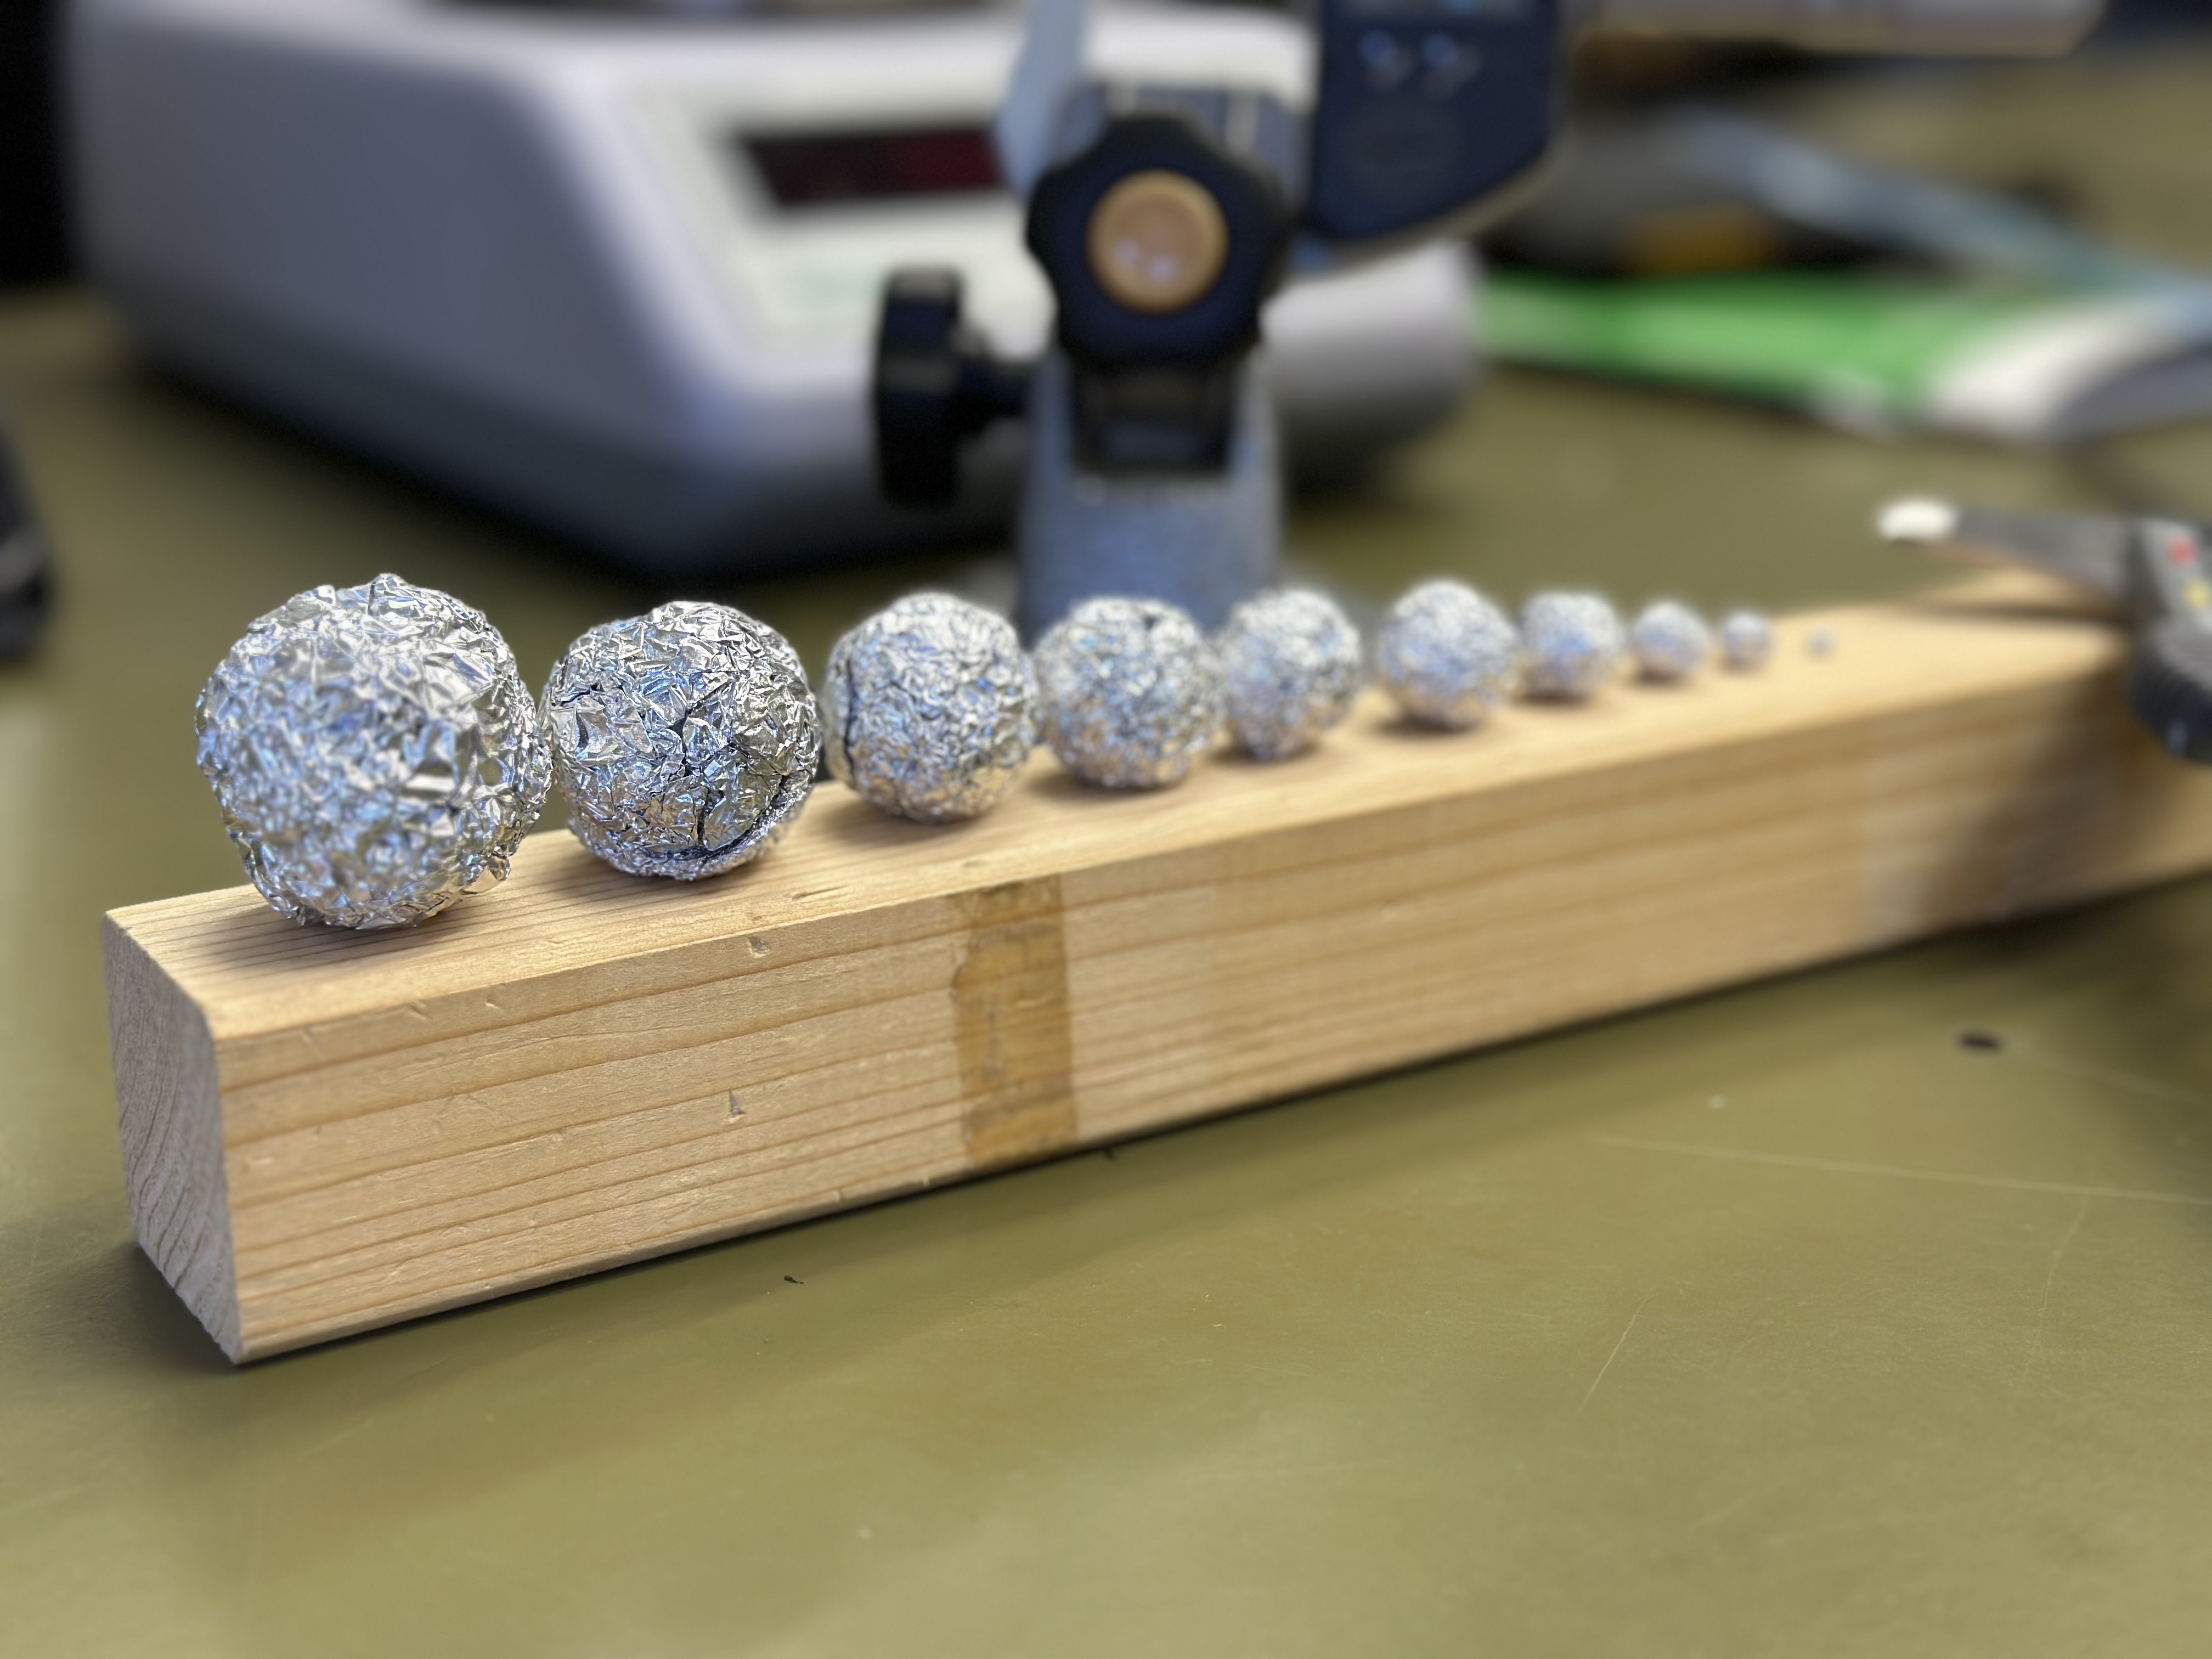
\includegraphics[width=\textwidth]{Tin_foil_balls.png}
    \end{minipage}%
    \hspace{0.05\textwidth} % Adds space between the images
    \begin{minipage}{0.45\textwidth}
        \centering
        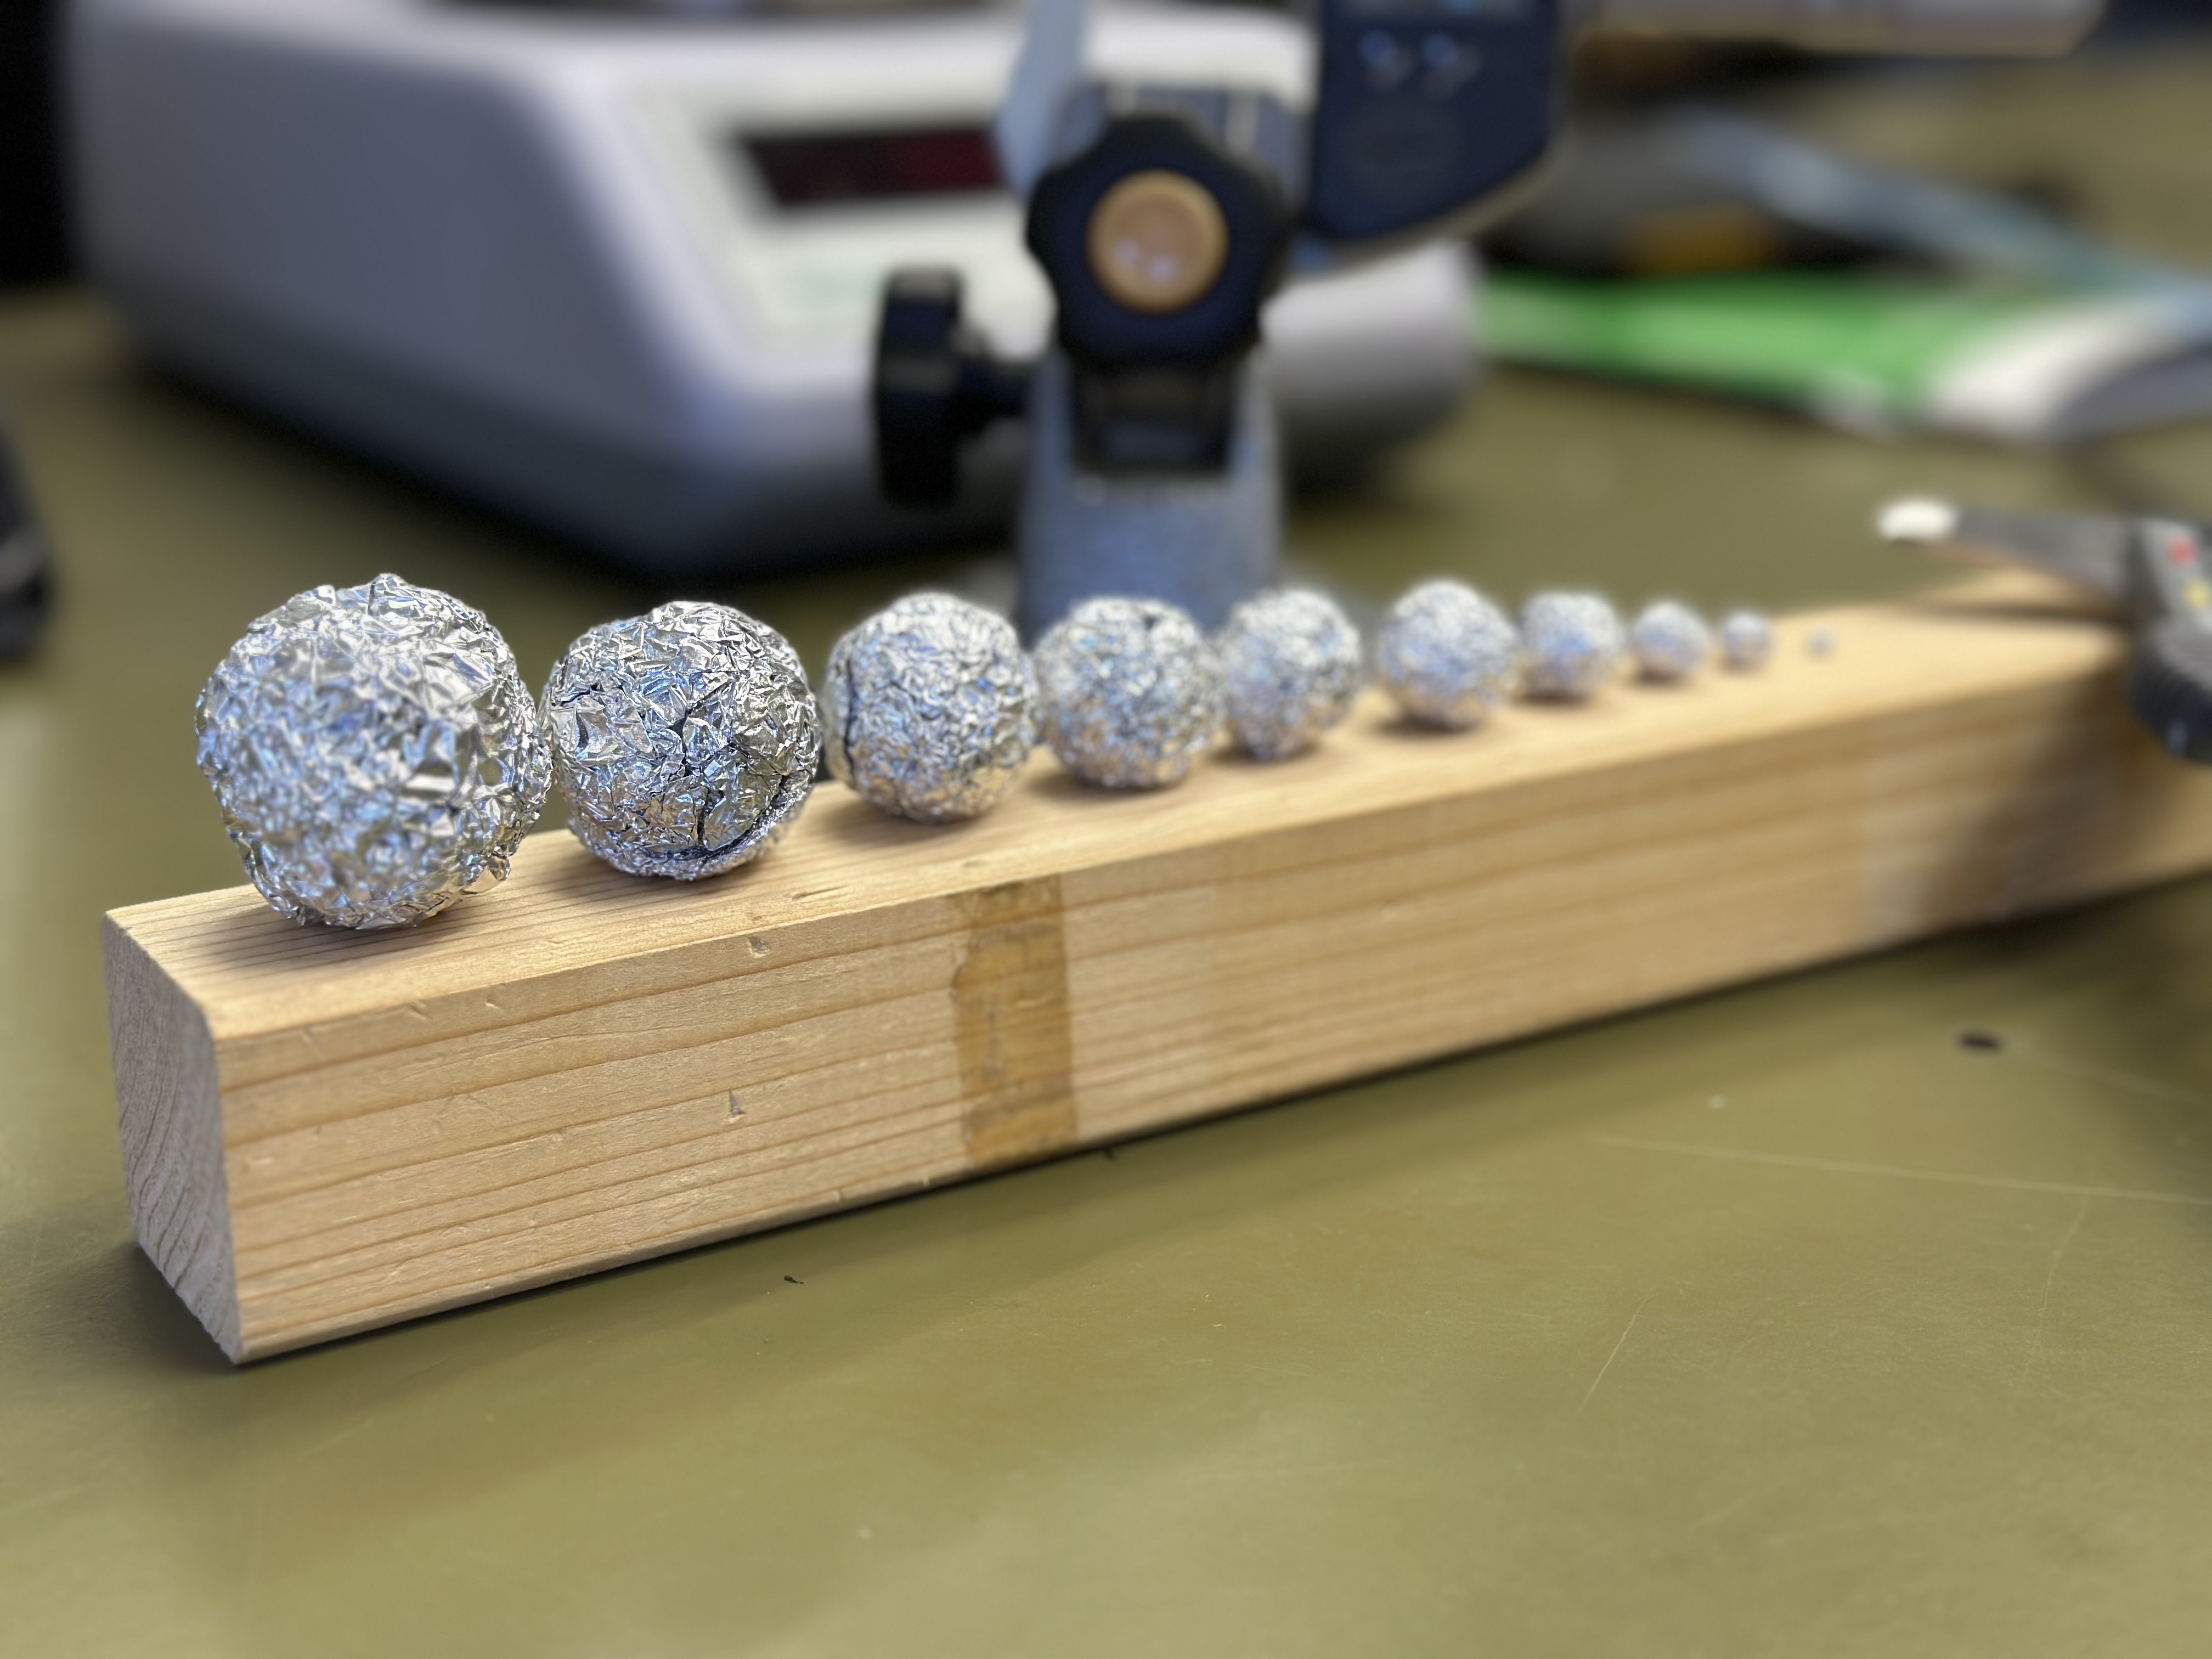
\includegraphics[width=\textwidth]{Tin_foil_balls.jpg}
    \end{minipage}
    
    \caption{Some of the tin foil balls we made, the caliber, and some squares of tin foil in the background.}
    \label{fig:tf_balls}
\end{figure}

Once finished, our last measurment is to collect the information of the linear dimension 
of each ball (its diameter). We use the caliber or the micrometer (depending on the size of the ball) to measure the diameter 
along three different axis. We put this data in an excel spreadsheet, too.

% Results (Graphs and Data)
\section{Results}\label{sec:results}
\subsection{Part 1: Aluminum Foil Squares}
The data collected from the aluminum foil squares is shown in Tables (\ref{tab:squares}) and (\ref{tab:balls}); for instance, as explained in the preceding section, 
for each square, we measured six times its linear dimension along different axis in order to reduce the error in the measurements. 
In the same way, while measuring the mass of the squares, we repeated the same procedure three times and the related data is shown 
in Table (\ref{tab:balls}).

\begin{table}[!ht]
    \centering
    \begin{tabular}{|c|c|c|c|}
    \hline
        \textbf{Square (cm)} & \( \overline{L} \pm \Delta L \) (cm) & \( \overline{m} \pm \Delta m \) (g) \\ \hline 
        \textbf{29x29} & 29.02 \(\pm\) 0.11 & 2.80 \(\pm\) 0.01 \\ \hline
        \textbf{26x26} & 26.02 \(\pm\) 0.13 & 2.28 \(\pm\) 0.01 \\ \hline
        \textbf{23x23} & 23.00 \(\pm\) 0.10 & 1.77 \(\pm\) 0.01 \\ \hline 
        \textbf{20x20} & 20.02 \(\pm\) 0.11 & 1.34 \(\pm\) 0.01 \\ \hline
        \textbf{17x17} & 17.02 \(\pm\) 0.11 & 0.97 \(\pm\) 0.01 \\ \hline
        \textbf{14x14} & 14.00 \(\pm\) 0.12 & 0.66 \(\pm\) 0.01 \\ \hline
        \textbf{11x11} & 11.00 \(\pm\) 0.10 & 0.40 \(\pm\) 0.01 \\ \hline
        \textbf{8x8}   & 7.98  \(\pm\) 0.11 & 0.21 \(\pm\) 0.01 \\ \hline
        \textbf{5x5}   & 5.00  \(\pm\) 0.10 & 0.08 \(\pm\) 0.01 \\ \hline
        \textbf{3x3}   & 3.00  \(\pm\) 0.10 & 0.02 \(\pm\) 0.01 \\ \hline
    \end{tabular}
    \caption{Measurements of Squares with Average Length and Mass with their respective uncertainties}
    \label{tab:squares}
\end{table}



\subsection{Part 2: Crumpled Aluminum foils}
\begin{table}[h!] 
    \centering
    \begin{tabular}{|c|c|c|c|}
    \hline
        \textbf{Square (cm)} & \( \overline{D} \pm \Delta D \) (mm) \\ \hline 
        \textbf{29x29} & 35.348 \(\pm\) 0.903              \\ \hline
        \textbf{26x26} & 29.245 \(\pm\) 0.881              \\ \hline
        \textbf{23x23} & 25.852 \(\pm\) 0.327              \\ \hline
        \textbf{20x20} & 23.304 \(\pm\) 1.319              \\ \hline
        \textbf{17x17} & 20.240 \(\pm\) 1.177              \\ \hline
        \textbf{14x14} & 18.170 \(\pm\) 0.720              \\ \hline
        \textbf{11x11} & 14.950 \(\pm\) 0.824              \\ \hline
        \textbf{8x8}   & 10.643 \(\pm\) 0.386              \\ \hline
        \textbf{5x5}   & 7.535  \(\pm\) 0.305              \\ \hline
        \textbf{3x3}   & 3.117 \(\pm\) 0.212               \\ \hline
    \end{tabular}
    \caption{Diameters values for each aluminum ball with their respective uncertainties}
    \label{tab:balls}
\end{table}

For the second part of the experiment, after having rolled up all the squares into balls, we proceeded to measure each diameter as explained in the previous section. The data collected from this measurements is reported in Table (\ref{tab:balls}).




\subsection{Remarks on the Data processing} 
We also compute the natural logarithm of the mean values of the mass, the diameter and the length shown in the tables above. The related errors are calculated using traditional methods of error propagation \cite{taylor-1997}, having taking into account the uncertainties of both casual and systematic nature. The results are shown in Table (\ref{tab:ln_errors}). These quantities will be useful in the following sections for the computation of the fractal dimension of the system using the well known Least Squares method.


\begin{table}[!ht]
    \centering
    \begin{tabular}{|c|c|c|c|c|c|}
    \hline
        \( \ln(L) \pm \Delta \ln(L) \) & \( \ln(m) \pm \Delta \ln(m) \) & \( \ln(D) \pm \Delta \ln(D) \) \\ \hline
        3.368 \(\pm\) 0.004 & 1.028 \(\pm\) 0.004 & 3.565 \(\pm\) 0.253 \\ \hline
        3.259 \(\pm\) 0.005 & 0.824 \(\pm\) 0.004 & 3.376 \(\pm\) 0.261 \\ \hline
        3.135 \(\pm\) 0.004 & 0.571 \(\pm\) 0.006 & 3.252 \(\pm\) 0.100 \\ \hline
        2.997 \(\pm\) 0.005 & 0.293 \(\pm\) 0.007 & 3.149 \(\pm\) 0.419 \\ \hline
        2.834 \(\pm\) 0.006 & -0.030 \(\pm\) 0.010 & 3.008 \(\pm\) 0.391 \\ \hline
        2.639 \(\pm\) 0.008 & -0.416 \(\pm\) 0.015 & 2.900 \(\pm\) 0.248 \\ \hline
        2.398 \(\pm\) 0.009 & -0.916 \(\pm\) 0.025 & 2.705 \(\pm\) 0.305 \\ \hline
        2.077 \(\pm\) 0.014 & -1.561 \(\pm\) 0.048 & 2.365 \(\pm\) 0.163 \\ \hline
        1.609 \(\pm\) 0.020 & -2.526 \(\pm\) 0.125 & 2.020 \(\pm\) 0.151 \\ \hline
        1.099 \(\pm\) 0.033 & -3.912 \(\pm\) 0.500 & 1.137 \(\pm\) 0.187 \\ \hline
    \end{tabular}
    \caption{Natural Logarithms and Their Errors}
    \label{tab:ln_errors}
\end{table}


% Discussion and Analysis
\section{Discussion and Analysis}

\subsection{Aluminum Foil Squares}
\par Once the data has been fully analysed, we can start by discussing the main results obtained from the experiment. 
In particular, studying the plot shown in Fig. (\ref{fig:mass_vs_length}) which describes the relationship between the mass of the aluminum 
squares and their linear dimension, we can easily observe (as expected) that the data is well represented by a power law.

\begin{figure}[h!] 
    \centering
    \includegraphics[width = 0.8\textwidth]{mass_vs_length.png}
    \caption{Mass vs Length of the Aluminum Squares}
    \label{fig:mass_vs_length}
\end{figure}

The power law obtained from the data is given by the the equation $M = 0.0034 L^{1.9928}$ where $M$ corresponds 
to the mass of the aluminum squares and $L$ to its linear dimension. The exponent of the power law in the previous equation is very close 
to $2$, which is the expected value for a two-dimensional object; infact, we obtain a value of $\alpha = 1.99 \pm 0.01$ for the 
exponent and for the parameter $k$ the fit provided a value of $k = 0.0034 \pm 0.0001 \, g/cm^3$ . This law was obtained numerically 
using the Python library \texttt{scipy} and the function \texttt{curve\_fit}, which uses a non-linear least squares method to compute these parameters. 
This is a very satisfactory result supported by the associated $R^2$ parameter, which validates the fit of the 
data to the expected power law.  

In addition, we can consider a different approach to the problem by using the Least Squares method to compute both parameters of the power law. With this aim, we calculate 
the natural logarithm of the general law $M = k L^{\alpha}$, obtaining 
\begin{equation}
    \ln(M) = \ln(k) + \alpha \ln(L),
\end{equation}
which clearly describe a linear dependence between the natural logarithm of the mass and the natural logarithm of the linear dimension. Using the data from Table (\ref{tab:ln_errors}), we can plot this relationship and compute the parameters $k$ and $\alpha$ using the Least Squares method. The results are shown in Fig. (\ref{fig:ln_mass_vs_ln_length}).
\begin{figure}[h!]
    \centering
    \includegraphics[width = 0.8\textwidth]{ln_mass_vs_ln_length.png}
    \caption{Natural logarithm of Mass vs Natural logarithm of Length of the Aluminum Squares. Alternative approach for the computation of the dimensionality parameters.}
    \label{fig:ln_mass_vs_ln_length}
\end{figure}

As expected, we found that the data is well represented by a linear function, whose parameters $\ln(k)$ and $\alpha$ correspond to the slope and the intercept of the line, respectively. 
The values obtained for these parameters are 
\begin{align}
    \ln(k) &= -6.07 \pm 0.11 \implies (k = 0.0020 \pm 0.0003) \, g/cm^3,\\ \notag
    \alpha &= 2.13 \pm  0.04.
\end{align}

These values are in perfect agreement with the ones obtained from the previous method, which validates the results obtained from the experiment.

\subsection{Crumpled Aluminum Foil Spheres}
On the other hand, for the second part of the experiment, we follow the same procedure as before, and now we study the relationship between the mass 
of the aluminum squares (now crumpled aluminum balls) and their linear dimension: the diameter. The plot shown in Fig. (\ref{fig:mass_vs_diameter}) 
describes this relationship and, as expected, the data is well represented by a power law whose parameters are $\alpha = 1.97 \pm 0.14$ and $k = 0.003 \pm 0.001$ $g/mm^3$. 
However, the exponent we obtained in this case contradicts our predictions since we expected a value ranging from $2$ to $3$. This discrepancy could be due to the fact 
that the balls were not rolled up uniformly, which could have affected the measurements of the diameter and consequently the results obtained from the experiment. Even if the $R^2$ parameter is very close to $1$, 
we can not consider the results obtained from this part of the experiment as satisfactory. 
We consider that, one possible way to improve these results, could be collecting more data regarding the diameter of each ball by measuring them across several more different axis. 

\begin{figure}[h!]
    \centering
    \includegraphics[width = 0.8\textwidth]{mass_vs_diameter.png}
    \caption{Mass vs Diameter of the Aluminum Balls. As expected, the data is well represented by a power law.}
    \label{fig:mass_vs_diameter}
\end{figure}

Finally, we compare the previous results with the ones obtained from the Least Squares method. The plot shown in Fig. (\ref{fig:ln_mass_vs_ln_diameter}) describes the relationship between the natural logarithm of the mass and the natural logarithm of the diameter of the aluminum balls.

\begin{figure}[h!]
    \centering
    \includegraphics[width = 0.8\textwidth]{ln_mass_vs_ln_diameter.png}
    \caption{Natural logarithm of Mass vs Natural logarithm of Diameter of the Aluminum Balls. Alternative approach for the computation of the dimensionality parameters.}
    \label{fig:ln_mass_vs_ln_diameter}
\end{figure}

As before, we use the Least Square method to compute the parameters of the power law we are interested in.
In Fig. (\ref{fig:ln_mass_vs_ln_diameter}), we show the linear law that best fits the data, whose parameters are 
\begin{align}
    \ln(k) &= -6.60 \pm 0.22 \implies k = (1.0 \pm 0.3) \, g/cm^3,  \\ \notag
    \alpha &= 2.16 \pm  0.08
\end{align}


These results are closer to the ones expected and we consider them more reliable than the ones obtained from the previous method.
 
\subsection{Further analysis and observations}\label{sec:Further_analysis}

We now make some comments about the results obtained in the previous section. In particular, 
since the parameters obtained from the power law and the linear regression for the second part of the 
experiments were not as satisfactory as expected, we decided to analyze the residuals of the experimental 
data 
\begin{equation}
    \textbf{Residuals} = \text{Experimental Data} - \text{Data predicted by the models}
\end{equation}

and the data predicted by the models (power law and linear regression). The results are shown in 
Fig. (\ref{fig:residuals}).

\begin{figure}[h!]
    \centering
    \includegraphics[width = 0.9\textwidth]{residuals.png}
    \caption{Residuals of the experimental data and the data predicted by the models.}
    \label{fig:residuals}
\end{figure} 
 
As we can see from these plots, in some cases there are some residuals that are not randomly distributed 
around the zero line (as we expected them to be). We also observed that these residuals correspond in general 
to the initial and final data points, the former with the highest uncertainty. We address 
this issue by excluding these data points from the analysis and repeating the calculations. The results obtained, 
for our surprise, were noticably better than the previous ones. For instance, for the second part of the experiment
we obtained a value of $\alpha = 2.47 \pm 0.07$ for the power law and using the linear regression the model provided 
a value of $\alpha = 2.38 \pm 0.08$. Since for the first part of the experiment our results were in agreement with the
expected values, we decided to keep the initial data points during the analysis but as an interesting result, we 
observed that if we do not include the data from the smallest aluminum square, the linear regression gives a value of 
alpha of $2.02 \pm 0.01$, which is closer to the expected value of $2$ than the one we obtained in the last section. 
We finally gather all the results obtained in the following table, 

\begin{table}[h!]
    \centering
    \caption{Summary of Results obtained from the experiment. The last two rows show the results described in section (\ref{sec:Further_analysis}).}
    \label{tab:summary_results}
    \begin{tabular}{|c|c|c|c|c|}
    \hline
    \textbf{Part} & \textbf{Method} & \textbf{$\alpha$}   \\ \hline
    Aluminum Square sheets & Power Law & $\alpha = 1.99 \pm 0.01$   \\ \hline
    Aluminum Square sheets & Linear Regression & $\alpha = 2.13 \pm 0.04$   \\ \hline
    Aluminum Spherical balls & Power Law & $\alpha = 1.97 \pm 0.14$  \\ \hline
    Aluminum Spherical balls & Linear Regression & $\alpha = 2.16 \pm 0.08$   \\ \hline
    Further Results 2.1 & Power Law & $\alpha = 2.47 \pm 0.07$  \\ \hline
    Further Results 2.2 & Linear Regression & $\alpha = 2.38 \pm 0.08$ \\ \hline
    \end{tabular}
    \end{table}
 



+ 
% Conclusion 
\section{Conclusion}\label{sec:conclusion}
The purpose of this experiment was to study the fractal dimension of two geometrically different objects: aluminum squares and aluminum tinfoil spheres, 
the later being neither completely solid nor completely hollow, and whose dimentionality we demonstrated, falls between 2 and 3. 
After following the procedure outlined in section (\ref{subsec:exp_procedure}), we were able to obtain and analyze the data.
In the first part of the experiment we demonstrated that the dimensionality of the aluminum squares is close to $2$, as expected.
However, the problem emerged when applying the same procedure to the aluminum spheres, where we obtained two significantly different values 
using differet methods. Is it possible to explain this discrepancy in the two values by noting that the balls were rolled up manually,
this means that it was impossible to roll them up in the same way, which could have affected the measurements of the diameter and consequently the results obtained from the experiment.
Finally, by analyzing the residuals of the experimental data, we found the first and the last data points to be "problematic", the former being the one with the highest uncertainty,
this means that we can obtain more reliable results by excluding these data points from the analysis and repeating the calculations, as we shown in Table \ref{tab:summary_results}.
In conclusion, we can say that the experiment was successful in demonstrating the fractal nature of the objects studied.
However, several aspects could be improved; the inconsistency in the results obtained from different methods highlights 
the need for more controlled conditions, particularly a better way to prepare the spheres. The manual rolling process introduced variability that likely affected the measurements. 
Finally, increasing the number of data points could have further enhanced the reliability of the experiment.
By addressing these areas, future experiments could yield more robust and reproducible results.

 
% References
\newpage
\printbibliography

\end{document}
